\documentclass[11pt,letterpape, fleqn]{article}
\usepackage[lmargin=1in,rmargin=1in,tmargin=1in,bmargin=1in]{geometry}

% -------------------
% Packages
% -------------------
\usepackage{
	amsmath,			% Math Environments
	amssymb,			% Extended Symbols
	enumerate,		% Enumerate Environments
	graphicx,			% Include Images    
	lastpage,			% Reference Lastpage
	multicol,			% Use Multi-columns
	multirow,			% Use Multi-rows
	siunitx
}

\graphicspath{{./images/}}

\usepackage{wrapfig}

% -------------------
% Font
% -------------------
\usepackage[T1]{fontenc}
\usepackage{charter}    


% -------------------
% Heading Commands
% -------------------
\newcommand{\class}{Mu Alpha Theta}
\newcommand{\term}{2022-2023}
\newcommand{\head}[4]{%
\thispagestyle{empty}
\vspace*{-0.5in}
\noindent\begin{tabular*}{\textwidth}{l @{\extracolsep{\fill}} r @{\extracolsep{6pt}} l}
	\textbf{#1} & \textbf{Name:} & \makebox[5.75cm]{\hrulefill} \\
	\textbf{#2} & & \\
	\textbf{\class:\; \term} & & \\
\end{tabular*} \\
\rule[2ex]{\textwidth}{2pt} %
}


% -------------------
% Commands
% -------------------
\newcommand{\prob}{\noindent\textbf{Problem. }}
\newcounter{problem}
\newcommand{\problem}{
	\stepcounter{problem}%
	\noindent \textbf{Problem \theproblem. }%
}
\newcommand{\pointproblem}[1]{
	\stepcounter{problem}%
	\noindent \textbf{Problem \theproblem.} (#1 points)\,%
}
\newcommand{\pspace}{\par\vspace{\baselineskip}}
\newcommand{\ds}{\displaystyle}


% -------------------
% Header & Footer
% -------------------
\usepackage{fancyhdr}

\fancypagestyle{pages}{
	%Headers
	\fancyhead[L]{}
	\fancyhead[C]{}
	\fancyhead[R]{}
\renewcommand{\headrulewidth}{0pt}
	%Footers
	\fancyfoot[L]{}
	\fancyfoot[C]{}
	\fancyfoot[R]{}
\renewcommand{\footrulewidth}{0.0pt}
}
\headheight=0pt
\footskip=14pt

\pagestyle{pages}


% -------------------
% Content
% -------------------

\begin{document}
\head{Worksheet \#5}{Date:}
\centering

% Question 1: 12pi (2002 AMC10)
\begin{minipage}{\textwidth}
	\problem

	\begin{wrapfigure}[11]{r}{0.4\textwidth}
		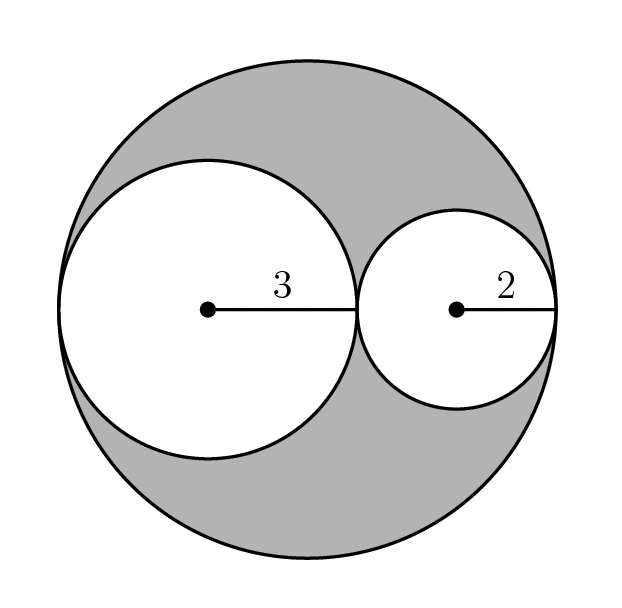
\includegraphics[width = 6cm]{images/q1.png}
   \end{wrapfigure}
   \noindent Circles of radius $2$ and $3$ are externally tangent and are circumscribed by a third circle, as shown in the figure. Find the area of the shaded region. Express your answer in terms of $\pi$.

    \vspace{7cm}
\end{minipage}

% Question 2: 18 (CEMC 2006 Pascal)
\begin{minipage}{\textwidth}
    \problem

	\begin{wrapfigure}[11]{l}{0.4\textwidth}
		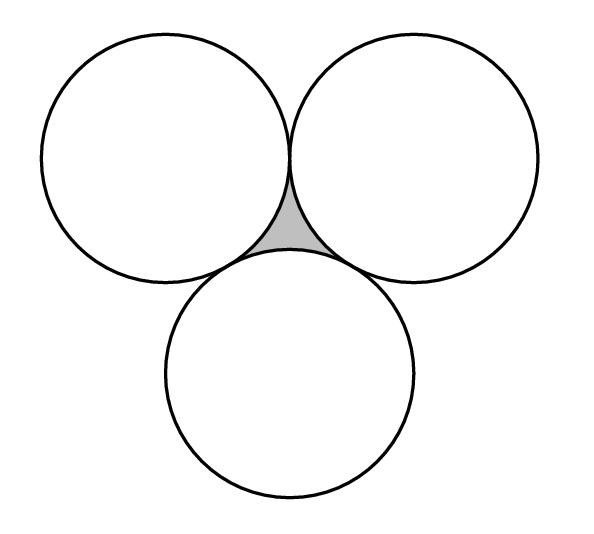
\includegraphics[width = 6cm]{images/q2.png}
   \end{wrapfigure}
   \noindent In the diagram, each of the three identical circles touch the other two. The circumference of each circle is 36. What is the \textbf{perimeter} of the shaded region?
	
   \vspace{7cm}
\end{minipage}

% Question 3: 2(pi - 2) = 2.28 (MathCounts 2004 Chapter Target)

\begin{minipage}{\textwidth}
    \problem

	\begin{wrapfigure}[11]{r}{0.5\textwidth}
		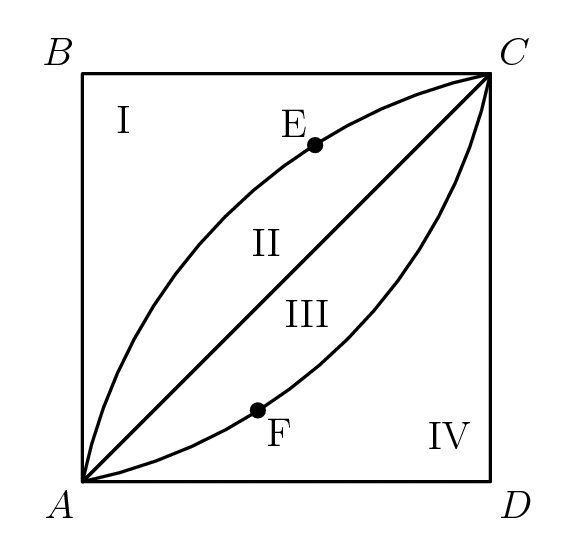
\includegraphics[width = 7cm]{images/q3.png}
   \end{wrapfigure}
   \noindent Quadrilateral $ABCD$ is a square. A circle with center $D$ has arc $AEC$. A circle with center $B$ has arc $AFC$. If $AB = 2$ cm, what is the total number of square centimeters in the football-shaped area of regions II and III combined? 

   \vspace{7cm}
\end{minipage}

% Question 4: pi (MathCounts 2008 Chapter Sprint)
\begin{minipage}{\textwidth}
    \problem

	\begin{wrapfigure}[11]{l}{0.5\textwidth}
		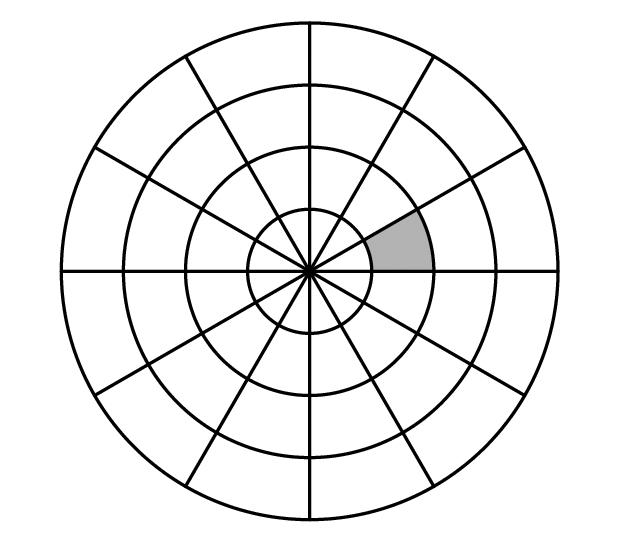
\includegraphics[width = 7cm]{images/q4.png}
   \end{wrapfigure}
   \noindent A decorative arrangement of floor tiles forms concentric circles, as shown in the figure below. The smallest circle has a radius of $2$ feet, and each successive circle has a radius $2$ feet longer. All the lines shown intersect at the center and form $12$ congruent central angles. What is the area of the shaded region? Express your answer in terms of $\pi$.

   \vspace{7cm}
\end{minipage}

% Question 5: 11 NOT 27 (MathCounts 2011 State Sprint)

\begin{minipage}{\textwidth}
    \problem

	\begin{wrapfigure}[11]{l}{0.5\textwidth}
		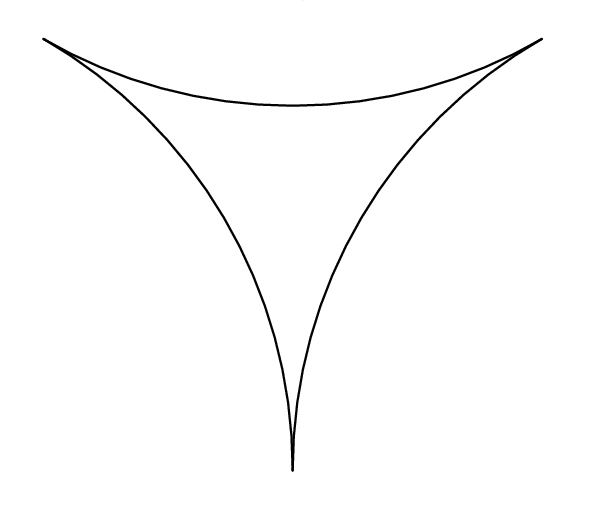
\includegraphics[width = 7cm]{images/q5.png}
   \end{wrapfigure}
   \noindent The region shown is bounded by the arcs of circles having radius $4$ units, having a central angle measure of $60$ degrees and intersecting at points of tangency. The area of the region can be expressed in the form $a\sqrt{b}+c\pi$ square units, where $\sqrt{b}$ is a radical in simplest form. What is the value of $a + b + c$?

   \vspace{7cm}
\end{minipage}




\vspace{6cm}
\end{document}
